\documentclass{article}
\usepackage{amsmath}
\usepackage{amssymb}
\usepackage{graphicx}
\usepackage{hyperref}
\usepackage[version=4]{mhchem}

\title{Example 2}
\date{}

\begin{document}
\maketitle

In \(\triangle A B C\), \(A N\) bisects \(\angle B A C, B N \perp A N . M N / / A C\). Prove that \(B M=\) MC.

Solution:
In the adjoining figure, \(B N\) is extended past \(N\) and meets \(A C\) at \(E\). Triangle \(B N A\) is congruent to \(\triangle E N A\), since \(\angle B A N=\angle E A N, A N=A N\) and \(\angle A N B=\angle A N E\) \(=90^{\circ}\).

Therefore \(N\) is the midpoint of \(B E\). Since \(M N / / A C\),\\
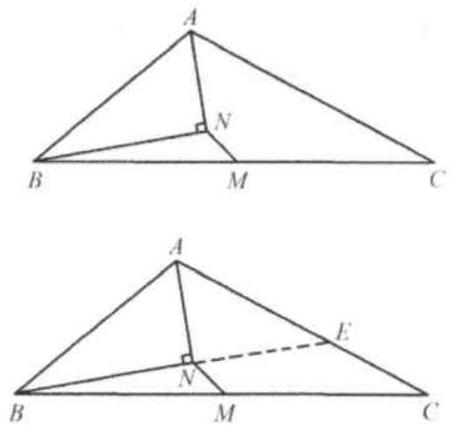
\includegraphics[width=\textwidth]{images/055(1).jpg} \(M N / / E C\). Thus \(M N\) is the midline of \(\triangle B C E\).\\
So \(B M=M C\).


\end{document}
